\documentclass[11pt]{article}
\usepackage[a4paper,margin=2.5cm]{geometry}
\usepackage{amsmath,amssymb,amsthm,graphicx,booktabs,xcolor}
\usepackage[colorlinks=true,linkcolor=blue!60!black,citecolor=blue!60!black,urlcolor=blue!60!black]{hyperref}
\usepackage{xurl}
\hypersetup{pdftitle={Thermodynamics of Scale},pdfauthor={Ruqing Chen}}
\setlength{\emergencystretch}{3em}
\graphicspath{{../figures/}{figures/}{./}}

\newtheorem{theorem}{Theorem}
\newtheorem{proposition}{Proposition}[section]
\newtheorem{corollary}{Corollary}[section]
\newtheorem{conjecture}{Conjecture}
\theoremstyle{remark}\newtheorem*{remark}{Remark}

\newcommand{\dd}{\mathrm{d}}
\newcommand{\Tr}{\mathrm{Tr}}
\newcommand{\Var}{\mathrm{Var}}
\newcommand{\RR}{\mathbb{R}}
\newcommand{\ZZ}{\mathbb{Z}}
\newcommand{\paperdoi}{10.5281/zenodo.23199122}

\title{Thermodynamics of Scale:\\
Entropic $c$-Functions, Data Processing,\\ Spectral Thermodynamics, Fluctuation Relations,\\
and the Arrow of Time}
\author{Ruqing Chen\\[2pt]
\small GUT Geoservice Inc., Montreal, Quebec, Canada\\
\small \href{mailto:ruqing@hotmail.com}{\texttt{ruqing@hotmail.com}}}
\date{\small DOI: \href{https://doi.org/\paperdoi}{\paperdoi}}

\begin{document}
\maketitle

\begin{abstract}
The irreversibility of the renormalization group (RG) is often described with thermodynamic words: information is
``lost'' under coarse-graining, $c$ ``decreases like an entropy'', scale behaves like a temperature, and the RG
arrow is compared with the arrow of time. We sort these statements into theorems, exact identities, standard
physics in a new setting, and conjecture, and we check each exact statement numerically.

First, the RG theorems ($c$, $F$, $a$) state that the relevant quantity \emph{decreases} from the ultraviolet to the
infrared. In the entropic proofs this follows from strong subadditivity together with Lorentz invariance, not from a
thermodynamic law. For a massive lattice Dirac fermion the Casini--Huerta function $c(\ell)=3\ell\,\dd S/\dd\ell$
decreases monotonically from its lattice value to zero, and at the critical point it reproduces $c=1$ up to the
finite-size chord factor $(\pi\ell/N)\cot(\pi\ell/N)$. Second, the monotonicity of relative entropy under quantum
channels yields a rigorous $H$-theorem for any RG map that is a channel with an invariant state. It is checked
on block restrictions of Gaussian fermion states. Third, if the heat-kernel time $\tau$ is read as an inverse
temperature on the Laplacian spectrum, then $S(\tau)=\ln P+\tau\langle\lambda\rangle=-D(\pi_\tau\Vert\bar\rho)$ is
non-increasing, and the heat capacity $C=\tau^2\Var(\lambda)$ obeys $C=\tfrac12 d_s-\tfrac12\,\dd d_s/\dd\ln\tau$.
On scaling plateaus the spectral dimension is therefore twice a heat capacity. For the hypercubic lattice $C$ is
given in closed form; it has a Schottky-type maximum $0.6799\,d$ and tends to the equipartition value $d/2$.
Fourth, a physical protocol that changes the correlation length of a lattice field in time obeys the Jarzynski and
Crooks relations exactly. We prove that the sudden-quench Jarzynski estimator has finite variance if and only if
every mode stiffens by more than a factor $1/2$ in $\omega^2$. For finite ramp times, an exact Riccati equation
for the tilted Gaussian density decides the question; it shows that the softening protocol keeps an infinite
variance at every simulated ramp time. Simulations of a stiffening protocol, combined with the Bennett acceptance ratio, recover $\Delta F$ to
within $0.015$.

Landauer's bound applies to physical erasure, not to the theorist's coarse-graining map. The identification of the
thermodynamic arrow of time with the RG arrow, suggested by dS/CFT and by holographic $c$-theorems, is formulated
as a conjecture together with what it does not explain: the low-entropy initial state.
\end{abstract}

\tableofcontents

%=====================================================================
\section{Introduction}
\label{sec:intro}

Wilson's renormalization group integrates out short-distance degrees of freedom, and the resulting flow
in the space of theories is irreversible in a precise sense: in two dimensions Zamolodchikov's
$c$-theorem~\cite{Zamolodchikov} provides a function that decreases along the flow and equals the Virasoro central
charge at fixed points. In four dimensions the corresponding statement for the Euler anomaly $a$ was conjectured by
Cardy~\cite{Cardy} and proved by Komargodski and Schwimmer~\cite{KS}. In three dimensions the $F$-theorem was proposed
in~\cite{JKPS} and proved by Casini and Huerta from entanglement entropy~\cite{CH2012}. In every case
\begin{equation}
c_{\rm UV}>c_{\rm IR},
\label{eq:cUVIR}
\end{equation}
with the inequality pointing from short to long distances.

This structure invites thermodynamic language: coarse-graining ``forgets'' information, $c$ counts degrees of
freedom like an entropy, the RG scale is a kind of temperature, and the direction of the flow resembles the
direction of time. Earlier work made parts of this precise. Gaite and O'Connor proposed an $H$-theorem for
field-theory entropy~\cite{GaiteOConnor}, and Bény and Osborne described RG maps as quantum channels and measured
information loss by distinguishability~\cite{BenyOsborne}. In holography the radial coordinate plays the role of
scale~\cite{FGPW,MyersSinha}, and in dS/CFT cosmological time is dual to RG scale~\cite{StromingerdS,StromingerInfl}.

Thermodynamic language is also easily over-extended. In this paper we separate four kinds of statements and
attach a numerical check to each exact one.
\begin{enumerate}
\item \emph{Theorems about the RG}, proved from quantum information inequalities (Section~\ref{sec:entropic}): the
entropic $c$-function, and an $H$-theorem from the data-processing inequality.
\item \emph{An exact identity} that makes ``scale as inverse temperature'' precise (Section~\ref{sec:spectral}).
\item \emph{Standard thermodynamics applied to scale}: Landauer's principle for physical coarse-graining devices
(Section~\ref{sec:landauer}) and the Jarzynski and Crooks relations for protocols that change a correlation
length in time (Section~\ref{sec:jarzynski}). Neither is a new law.
\item \emph{A conjecture} that the thermodynamic arrow of time and the RG arrow coincide
(Section~\ref{sec:arrow}).
\end{enumerate}
From Ref.~\cite{Chen2026_qgc} we use the identity $d_s(\tau)=2\tau\langle\lambda\rangle_\tau$ for the spectral dimension.

All numbers below are produced by a single script, \texttt{scale\_thermodynamics.py}, whose output is reproduced in
the accompanying repository. Figure~\ref{fig:main} summarises the numerical results.

\begin{figure}[t]
\centering
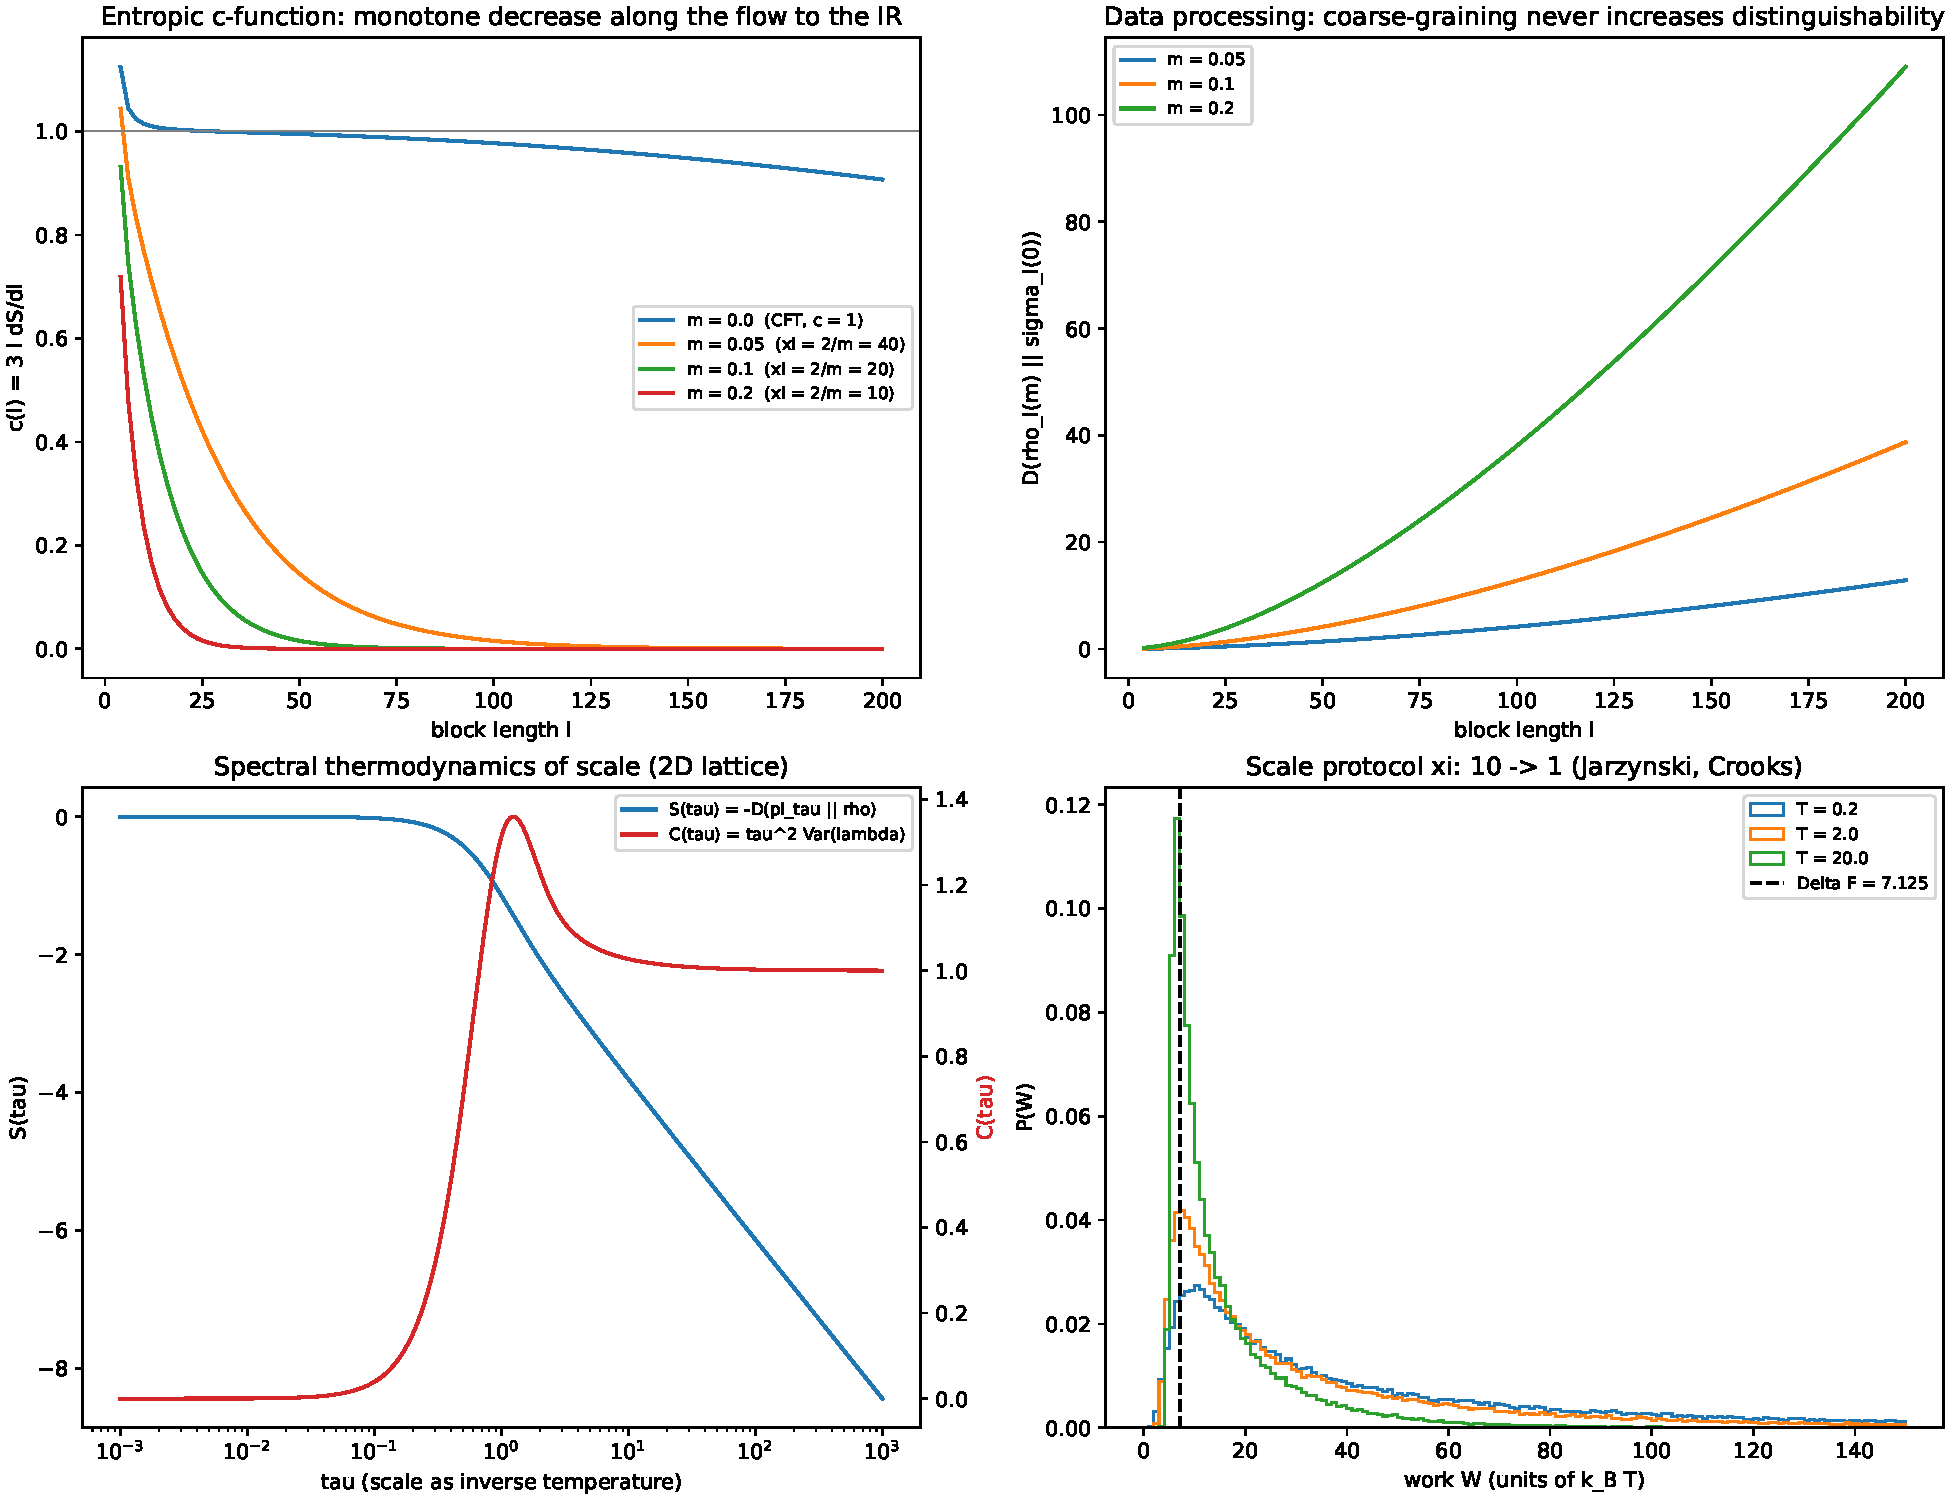
\includegraphics[width=\textwidth]{scale_thermodynamics.pdf}
\caption{Four exact statements, checked numerically.
\emph{Top left:} entropic $c$-function $c(\ell)=3\ell\,\dd S/\dd\ell$ of the half-filled lattice Dirac fermion
($N=1200$) for several masses; the correlation length is $\xi=2/m$ (Section~\ref{sec:cfunction}).
\emph{Top right:} relative entropy between the massive and massless reduced states, non-decreasing in the block
length as required by data processing (Section~\ref{sec:dpi}).
\emph{Bottom left:} spectral entropy $S(\tau)=-D(\pi_\tau\Vert\bar\rho)$ and heat capacity $C(\tau)$ of the
two-dimensional square lattice (Section~\ref{sec:spectral}).
\emph{Bottom right:} work distributions for the protocol $m^2:0.01\to1$ (correlation length $10\to1$) of a Gaussian
lattice field, for three durations $T$, with the exact $\Delta F$ (Section~\ref{sec:jarzynski}).}
\label{fig:main}
\end{figure}

%=====================================================================
\section{Irreversibility of the RG from entropy inequalities}
\label{sec:entropic}

\subsection{\texorpdfstring{The entropic $c$-function}{The entropic c-function}}
\label{sec:cfunction}

Let $S(r)$ be the entanglement entropy of an interval of length $r$ in the vacuum of a Lorentz-invariant
$(1+1)$-dimensional QFT. Casini and Huerta~\cite{CH2004} defined
\begin{equation}
c(r)=3r\,\frac{\dd S}{\dd r}
\label{eq:cr}
\end{equation}
(their normalisation differs by the factor $3$) and proved that
\begin{equation}
\frac{\dd c}{\dd r}=3\bigl(rS''(r)+S'(r)\bigr)\le0 .
\label{eq:dcdr}
\end{equation}
At a fixed point, $S=\tfrac c3\ln(r/\epsilon)$~\cite{HLW,CalabreseCardy} and $c(r)$ equals the central charge. The
proof uses only two ingredients. The first is strong subadditivity (SSA)~\cite{LiebRuskai},
\begin{equation}
S(AB)+S(BC)\ge S(B)+S(ABC),
\label{eq:ssa}
\end{equation}
applied to intervals that are boosted relative to each other. The second is Lorentz invariance, which makes $S$
depend only on the proper length of an interval. The irreversibility of the RG is therefore a statement about
quantum correlations in the vacuum and needs no thermodynamic hypothesis. The same strategy, with the Markov
property of the conformal vacuum, gives the $F$-theorem~\cite{CH2012} and the $a$-theorem~\cite{CTT}.

\begin{remark}
The direction of~\eqref{eq:cUVIR} is essential, and the thermodynamic analogy can mislead here. Under coarse-graining
$c$ \emph{decreases}, whereas thermodynamic entropy increases. The gradient-flow form
$\beta^i\partial_i c=-12\,\beta^i\beta^jG_{ij}$, with a positive metric $G_{ij}$, is established in conformal
perturbation theory~\cite{Zamolodchikov}. In general only the inequality between fixed points and the monotonicity
of a suitable $c$-function are proved.
\end{remark}

\paragraph{Lattice check.}
Consider the periodic chain of $N$ sites at half filling,
\begin{equation}
H=-\sum_j\bigl(c_j^\dagger c_{j+1}+\text{h.c.}\bigr)+m\sum_j(-1)^jn_j .
\label{eq:chain}
\end{equation}
Its single-particle spectrum is $\pm\sqrt{4\cos^2k+m^2}$. The low-energy theory is a Dirac fermion with velocity
$v=2$ and mass gap $m$, and the correlation length is $\xi=1/\operatorname{arsinh}(m/2)\simeq2/m$. Block
entropies follow from the eigenvalues of the restricted correlation matrix $C_{ij}=\langle c_i^\dagger
c_j\rangle$~\cite{Peschel} (Appendix~\ref{app:methods}). We evaluate~\eqref{eq:cr} by a central difference of step
$2$ on even block lengths, which removes the parity oscillations of the half-filled chain.

For $N=1200$ and $\ell=4,\dots,200$ we find the following (Figure~\ref{fig:main}, top left).
\begin{itemize}
\item At $m=0$, $c(200)=0.907$. This matches the finite-size prediction $c\,(\pi\ell/N)\cot(\pi\ell/N)=0.9069$ that
follows from $S=\tfrac13\ln[(N/\pi)\sin(\pi\ell/N)]+\text{const}$~\cite{CalabreseCardy} with $c=1$. The initial
value $c(4)=1.125$ is a lattice effect.
\item For $m=0.05,0.1,0.2$, $c(\ell)$ decreases monotonically from $1.044$, $0.931$ and $0.719$ to below $10^{-3}$.
The largest increment between successive points is at most $10^{-5}$, i.e.\ at the level of round-off.
\item The lattice form of SSA, $S(\ell+2)+S(\ell-2)-2S(\ell)\le0$, holds for every $\ell$. The largest values are
$-3.7\times10^{-5}$, $-4.9\times10^{-8}$, $-5.3\times10^{-12}$ and $+6.8\times10^{-13}$ (round-off).
\end{itemize}

\begin{remark}
On a lattice, SSA and translation invariance give only the concavity of $S(\ell)$, i.e.\ that $c(\ell)/\ell$ is
non-increasing. The monotonicity of $c(\ell)$ itself needs the Lorentz invariance of the continuum limit, so on the
lattice it is a property of this model and not a theorem.
\end{remark}

\subsection{\texorpdfstring{Data processing and an $H$-theorem for RG channels}{Data processing and an H-theorem for RG channels}}
\label{sec:dpi}

The rigorous version of ``coarse-graining loses information'' is the monotonicity of the relative entropy
$D(\rho\Vert\sigma)=\Tr\rho(\ln\rho-\ln\sigma)$ under completely positive trace-preserving maps (channels).

\begin{proposition}[Data processing~\cite{Lindblad,Uhlmann}]
\label{prop:dpi}
For every channel $\Phi$ and all states $\rho,\sigma$, $D(\Phi(\rho)\Vert\Phi(\sigma))\le D(\rho\Vert\sigma)$.
\end{proposition}

\begin{corollary}[$H$-theorem for RG channels]
\label{cor:H}
Let $\Phi$ be a channel on a fixed algebra of observables with an invariant state, $\Phi(\sigma_*)=\sigma_*$.
Then for every initial state $\rho$ the sequence $n\mapsto D(\Phi^n(\rho)\Vert\sigma_*)$ is non-increasing.
\end{corollary}

\begin{proof}
Apply Proposition~\ref{prop:dpi} with $\sigma=\sigma_*$:
$D(\Phi^{n+1}(\rho)\Vert\sigma_*)=D(\Phi(\Phi^n\rho)\Vert\Phi(\sigma_*))\le D(\Phi^n\rho\Vert\sigma_*)$.
\end{proof}

This is the exact sense in which an RG transformation is irreversible: if one step of the RG is a channel and the
fixed point is a state invariant under it, distinguishability from the fixed point can only decrease. Scale-invariant
MERA tensor networks provide examples. Their transfer (descending) maps are channels whose fixed points are
the scale-invariant reduced density matrices, and the rate of convergence encodes critical exponents~\cite{GMF}. The
corollary does not give strict decrease, and it gives a Lyapunov function relative to a chosen reference state, not
an intrinsic quantity of the theory such as $c$. The two statements are complementary: the $c$-theorem needs Lorentz
invariance but no reference state, and the $H$-theorem needs a channel and a fixed point but no symmetry.

\paragraph{Check.}
Let $\rho_\ell(m)$ be the ground state of~\eqref{eq:chain} restricted to a block of $\ell$ sites and $\sigma_\ell$
the restriction of the massless ground state. Restriction from $\ell+2$ to $\ell$ sites is a partial trace, so
Proposition~\ref{prop:dpi} requires $D(\rho_\ell\Vert\sigma_\ell)$ to be non-decreasing in $\ell$. For Gaussian states
the relative entropy is given by the correlation matrices (Appendix~\ref{app:methods}). We find
$D(\rho_\ell\Vert\sigma_\ell)$ rising from $0.025$, $0.072$, $0.197$ at $\ell=4$ to $12.85$, $38.73$, $109.0$ at
$\ell=200$ for $m=0.05,0.1,0.2$. The smallest increments are $+0.023$, $+0.064$ and $+0.17$
(Figure~\ref{fig:main}, top right).

%=====================================================================
\section{Spectral thermodynamics of scale}
\label{sec:spectral}

``Scale temperature'' becomes exact once the heat-kernel time is read as an inverse temperature. Let $\Delta$ be
a Laplacian on a graph with $V$ vertices and eigenvalues $\lambda_1,\dots,\lambda_V$, let $\bar\rho$ be the uniform
distribution on the spectrum, and let
\begin{equation}
P(\tau)=\frac1V\Tr e^{-\tau\Delta},\qquad
\pi_\tau(i)=\frac{e^{-\tau\lambda_i}}{V P(\tau)},\qquad
\langle f\rangle_\tau=\sum_i\pi_\tau(i)f(\lambda_i).
\label{eq:gibbs}
\end{equation}
$P$ is the return probability of the diffusion and, at the same time, the partition function of a canonical
ensemble on the spectrum at inverse temperature $\tau$. The spectral dimension of~\cite{Chen2026_qgc} is
$d_s=-2\,\dd\ln P/\dd\ln\tau=2\tau\langle\lambda\rangle_\tau$.

\begin{proposition}
\label{prop:spectral}
Define $S(\tau)=\ln P(\tau)+\tau\langle\lambda\rangle_\tau$ and $C(\tau)=\tau^2\Var_\tau(\lambda)$. Then
\begin{align}
S(\tau)&=-D(\pi_\tau\Vert\bar\rho)=H(\pi_\tau)-\ln V\le0, \label{eq:S}\\
\frac{\dd S}{\dd\tau}&=-\tau\Var_\tau(\lambda)\le0, \label{eq:dS}\\
C(\tau)&=\frac{d_s}{2}-\frac12\frac{\dd d_s}{\dd\ln\tau}\ \ge0 . \label{eq:C}
\end{align}
Moreover $-\ln P(\tau)=\min_p\bigl[\tau\,\mathbb E_p\lambda-H(p)+\ln V\bigr]$, with the minimum attained at
$p=\pi_\tau$ (Gibbs variational principle), so $-\ln P$ is $\tau$ times a free energy.
\end{proposition}

\begin{proof}
From~\eqref{eq:gibbs}, $\ln(V\pi_\tau(i))=-\tau\lambda_i-\ln P$, so $D(\pi_\tau\Vert\bar\rho)=\sum_i\pi_\tau(i)\ln
(V\pi_\tau(i))=-\tau\langle\lambda\rangle-\ln P=-S$; this also equals $\ln V-H(\pi_\tau)$. Next,
$\dd\ln P/\dd\tau=-\langle\lambda\rangle$ and $\dd\langle\lambda\rangle/\dd\tau=-\Var(\lambda)$, so
$\dd S/\dd\tau=-\langle\lambda\rangle+\langle\lambda\rangle-\tau\Var(\lambda)$. Finally,
$\dd d_s/\dd\ln\tau=\tau\,\dd(2\tau\langle\lambda\rangle)/\dd\tau=d_s-2\tau^2\Var(\lambda)=d_s-2C$. The variational
statement is the non-negativity of $D(p\Vert\pi_\tau)=\tau\mathbb E_p\lambda-H(p)+\ln V+\ln P$.
\end{proof}

\begin{corollary}[Dimension as heat capacity]
\label{cor:equipartition}
On a scaling plateau where $d_s$ is constant, $d_s=2C$. In flat $\RR^d$, $C=d/2$ exactly: each dimension
contributes $1/2$, as in equipartition.
\end{corollary}

\paragraph{Infinite lattices.}
On an infinite graph such as $\ZZ^d$ there is no uniform distribution on the eigenvalues, but none is needed. The
uniform distributions on the spectra of the tori $(\ZZ/n\ZZ)^d$ converge weakly to the density-of-states measure
$\mu$, a probability measure on $[0,4d]$. Replacing $\bar\rho$ by $\mu$ and $\pi_\tau$ by $\dd\pi_\tau=e^{-\tau\lambda}\dd\mu/P$,
$P(\tau)=\int e^{-\tau\lambda}\dd\mu(\lambda)$ is the return probability per site. Proposition~\ref{prop:spectral}
then holds verbatim with $S(\tau)=-D(\pi_\tau\Vert\mu)$, which is finite. Only the form $H(\pi_\tau)-\ln V$ has no
limit, because each of its two terms diverges. No divergent constant needs to be subtracted.

\paragraph{Hypercubic lattice.}
For $\ZZ^d$ with unit spacing, $P=(e^{-x}I_0(x))^d$ with $x=2\tau$~\cite{Chen2026_qgc}. Writing $r=I_1(x)/I_0(x)$
and using $r'=1-r/x-r^2$,
\begin{equation}
\langle\lambda\rangle_\tau=2d(1-r),\qquad
C(\tau)=d\,x^2\Bigl(1-\frac rx-r^2\Bigr),
\label{eq:Clattice}
\end{equation}
with $C\simeq2d\tau^2$ as $\tau\to0$ and $C\to d/2$ as $\tau\to\infty$. Because the factors are independent, $C/d$
does not depend on $d$. Its maximum is $C=0.6799\,d$ at $\tau=1.252$ (Figure~\ref{fig:main}, bottom left). This is
a Schottky-type anomaly caused by the band edge and the bounded spectrum. By~\eqref{eq:C} it is the
thermodynamic counterpart of the overshoot $\max d_s=1.2178\,d$ found in~\cite{Chen2026_qgc}. For $d=2$ the script
confirms~\eqref{eq:C} to $3\times10^{-4}$ (finite-difference error). It also confirms $\dd S/\dd\tau\le0$ and the
large-$\tau$ asymptote $S\simeq-\tfrac d2\ln(4\pi\tau)+\tfrac d2$, which gives $S(10^3)=-8.439$.

\begin{remark}
Proposition~\ref{prop:spectral} is an exact dictionary, but its monotonicity is the elementary fact that a canonical
ensemble loses entropy when it is cooled. It does not provide a dynamical arrow: $\tau$ is a resolution parameter,
the Euclidean proper time of the diffusion, and not physical time. Its content is that the thermodynamic response
of the spectrum, $C$, measures dimension.
\end{remark}

%=====================================================================
\section{What Landauer's principle does and does not say}
\label{sec:landauer}

Landauer's principle~\cite{Landauer,Bennett82} bounds the heat that a \emph{physical} process must dissipate when it
erases information stored in a physical memory. In the precise form of Reeb and Wolf~\cite{ReebWolf}, a system in
state $\rho_S$ that interacts unitarily with a bath initially in a Gibbs state at temperature $T$ dissipates heat
\begin{equation}
\langle Q\rangle\ge k_BT\,\bigl[S(\rho_S)-S(\rho_S')\bigr],
\label{eq:landauer}
\end{equation}
where $\rho_S'$ is the final state of the system. Erasing one bit therefore costs at least $k_BT\ln2$, which has been
confirmed experimentally~\cite{Berut}.

Three consequences follow for RG.
\begin{enumerate}
\item The RG of a theorist is a map between descriptions and does not act on a physical system in contact with a
bath, so it costs no energy. Statements such as ``every RG step dissipates $k_BT\ln2$ per discarded degree of
freedom'' have no basis.
\item If a device physically implements a coarse-graining, for example a detector that records block averages and
resets its fine-grained registers, then~\eqref{eq:landauer} applies to the device's memory with the temperature of
its bath.
\item Coarse-graining by partial trace may increase or decrease the von Neumann entropy. For example, a block of an
entangled pure state has positive entropy. The relevant invariant statement is the data-processing inequality of
Section~\ref{sec:dpi}, not a sign of $\Delta S$.
\end{enumerate}

%=====================================================================
\section{Fluctuation relations for a physical scale protocol}
\label{sec:jarzynski}

The Jarzynski equality~\cite{Jarzynski97} and the Crooks relation~\cite{Crooks} require a physical system driven
by a time-dependent control parameter. The RG flow itself is not such a protocol. A physical protocol that changes
the \emph{scale} of a system is, however, easy to construct: change the mass, and hence the correlation length, of
a field in time. The standard relations then hold, and in this sense they apply to scale. We treat a classical
field. For quantum systems, work is defined by two projective energy measurements and is not an
observable~\cite{TLH}. The statistics of the work done by quenching a parameter of a quantum many-body system, such
as the transverse field of the Ising chain, are related to the Loschmidt echo~\cite{Silva}. A quantum version of the
protocol below would be described in that framework.

\paragraph{Model.}
Let $\phi\in\RR^L$ be a field on a ring with
\begin{equation}
H_t(\phi)=\tfrac12\,\phi\cdot\bigl(-\Delta+m^2(t)\bigr)\phi,\qquad
\dd\phi=-\nabla H_t\,\dd t+\sqrt2\,\dd B_t
\label{eq:langevin}
\end{equation}
(overdamped Langevin dynamics, $k_BT=1$), with $m^2(t)$ ramped linearly from $m_i^2$ to $m_f^2$ over a time $T$.
The work is $W=\int_0^T\partial_tH_t\,\dd t=\tfrac12\int_0^T\dot{m}^2|\phi|^2\,\dd t$. In normal modes with
$q_k^2=4\sin^2(\pi k/L)$ and $\omega_k^2=q_k^2+m^2$, the free-energy difference is
\begin{equation}
\Delta F=\frac12\sum_{k=0}^{L-1}\ln\frac{q_k^2+m_f^2}{q_k^2+m_i^2},
\label{eq:dF}
\end{equation}
and
\begin{equation}
\langle e^{-W}\rangle=e^{-\Delta F},\qquad
\frac{P_F(W)}{P_R(-W)}=e^{W-\Delta F}.
\label{eq:jc}
\end{equation}
The lattice correlation length $\xi=1/\operatorname{arcosh}(1+m^2/2)$ changes from $10.0$ to $1.04$ for
$m^2:0.01\to1$.

\paragraph{Variance of the estimator.}
The exponential average converges poorly when it is dominated by rare trajectories~\cite{Jarzynski2006}. For
quadratic Hamiltonians this can be decided exactly in the sudden limit.

\begin{proposition}
\label{prop:variance}
For a sudden quench $m_i^2\to m_f^2$ from equilibrium, the estimator $e^{-W}$ has finite variance if and only if
$R_k=\omega_{f,k}^2/\omega_{i,k}^2>1/2$ for every mode $k$. In that case its relative variance is
$\prod_kR_k(2R_k-1)^{-1/2}-1$.
\end{proposition}

\begin{proof}
For a sudden quench, $W=\tfrac12(m_f^2-m_i^2)\sum_k\phi_k^2$ with independent $\phi_k\sim\mathcal N(0,\omega_{i,k}^{-2})$.
For $Z\sim\mathcal N(0,s^2)$, $\mathbb E\,e^{-aZ^2}=(1+2as^2)^{-1/2}$ if $1+2as^2>0$ and $+\infty$ otherwise. With
$a=m_f^2-m_i^2$ and $s^2=\omega_{i,k}^{-2}$, this gives $\mathbb E\,e^{-2W}=\prod_k(2R_k-1)^{-1/2}$ when all $R_k>1/2$,
and $+\infty$ otherwise. Dividing by $(\mathbb E\,e^{-W})^2=\prod_kR_k^{-1}$ gives the relative variance.
\end{proof}

For our ring ($L=16$) the forward (stiffening) protocol has $\min_kR_k=1.25$ and a sudden-limit relative variance of
$73.6$. The reverse (softening) protocol has $R_0=0.01<1/2$, so its sudden-limit estimator has infinite variance.

\paragraph{Finite ramp times.}
One might expect a finite switching time to restore a finite variance. For Gaussian dynamics this question can be
decided exactly.

\begin{proposition}
\label{prop:riccati}
For the dynamics~\eqref{eq:langevin} with a linear ramp of rate $\dot m^2$, $\mathbb E\,e^{-2W}<\infty$ if and only if,
for every mode $k$, the solution of
\begin{equation}
\dot b_k=2\omega_k^2(t)\,b_k-2b_k^2+2\dot m^2,\qquad b_k(0)=\omega_{i,k}^2,
\label{eq:riccati}
\end{equation}
stays positive on $[0,T]$. A positive adiabatic branch $b=\tfrac12\bigl(\omega^2+\sqrt{\omega^4+4\dot m^2}\bigr)$
exists only while $\omega_k^4\ge4|\dot m^2|$.
\end{proposition}

\begin{proof}
The tilted density $\tilde\rho(\phi_k,t)=\mathbb E[\delta(\phi_k(t)-\phi_k)\,e^{-2W_k(t)}]$ obeys, by the
Feynman--Kac formula, $\partial_t\tilde\rho=\partial_\phi(\omega_k^2\phi\tilde\rho)+\partial_\phi^2\tilde\rho
-\dot m^2\phi^2\tilde\rho$. The Gaussian ansatz $\tilde\rho=A(t)\,e^{-b(t)\phi^2/2}$ solves it if $b$
obeys~\eqref{eq:riccati} and $\dot A/A=\omega_k^2-b$. The total weight $\mathbb E\,e^{-2W_k}=A\sqrt{2\pi/b}$ is finite if
and only if $b$ stays positive; once $b$ reaches $0$ the tilted density is no longer normalisable. The adiabatic
branch is the positive root of the right-hand side of~\eqref{eq:riccati}.
\end{proof}

For softening ramps $\dot m^2<0$ pushes $b$ down. For our reverse protocol the adiabatic branch of the $k=0$ mode
disappears at the end of the ramp unless $T\ge4|\Delta m^2|/\omega_{\min}^4\approx4\times10^4$. For the discrete
protocol actually simulated, the same propagation is exact: each switch adds $2\Delta m^2$ to $b$, and each relaxation
step propagates the variance exactly. It gives an infinite second moment for the reverse protocol at $T=0.2$, $2$ and
$20$. The divergence is therefore not an artefact of the sudden limit. The weight $e^{-W}$ grows with $|\phi|^2$
when $\dot m^2<0$, and it grows faster than the Gaussian tail of the stiff initial ensemble decays. This is why a
first attempt that used the softening direction as the forward protocol gave estimates biased by more than one
unit. For the forward protocol the same calculation gives relative variances $56.7$, $20.8$ and $4.67$. With
$M=10^5$ these predict standard errors $0.024$, $0.014$ and $0.0068$, in agreement with the observed ones in
Table~\ref{tab:jc}. Estimates of $\Delta F$ should therefore be taken from the stiffening direction, or from the
Bennett acceptance ratio~\cite{BAR,Shirts}, which combines both directions optimally.

\paragraph{Simulation.}
We integrate~\eqref{eq:langevin} exactly, mode by mode, using the Ornstein--Uhlenbeck propagator over $400$ steps, for
$M=10^5$ trajectories in each direction. The exact value is $\Delta F=7.1254$. Table~\ref{tab:jc} shows that the
Jarzynski estimates agree with it within one standard error, that the Crooks slope is $1$ to within $2\%$, and that
the Bennett estimate agrees to within $0.008$. The dissipated work $\langle W\rangle-\Delta F$ is positive and
decreases towards the quasi-static limit, as the second law requires (Figure~\ref{fig:main}, bottom right).

\begin{table}[h]
\centering
\caption{Scale protocol $m^2:0.01\to1$ on a ring of $L=16$ sites, $M=10^5$ trajectories per direction. Exact
$\Delta F=7.1254$. The Crooks slope is the fitted slope of $\ln[P_F(W)/P_R(-W)]$ against $W$, expected to be $1$.}
\label{tab:jc}
\begin{tabular}{rrrrrr}
\toprule
$T$ & $\langle W\rangle$ & $\langle W\rangle-\Delta F$ & Jarzynski & Crooks slope & Bennett \\
\midrule
$0.2$ & $55.68$ & $48.56$ & $7.140\pm0.023$ & $0.995$ & $7.131$ \\
$2$ & $36.76$ & $29.63$ & $7.139\pm0.015$ & $0.981$ & $7.133$ \\
$20$ & $15.81$ & $8.69$ & $7.126\pm0.007$ & $1.003$ & $7.122$ \\
\bottomrule
\end{tabular}
\end{table}

%=====================================================================
\section{The RG arrow and the arrow of time}
\label{sec:arrow}

The statements so far are theorems or exact identities. The relation between the RG arrow and the arrow of time
is of a different kind, and we state what is established before formulating a conjecture.

\paragraph{Established.}
(i) The RG is irreversible in the sense of Sections~\ref{sec:cfunction} and~\ref{sec:dpi}.
(ii) In holographic RG flows the radial coordinate of the bulk acts as the scale. A $c$-function built from the
warp factor is monotone whenever the bulk matter satisfies the null energy condition~\cite{FGPW,MyersSinha}.
(iii) In dS/CFT, if it exists, the late-time boundary of de Sitter space carries a Euclidean CFT, and cosmological
time evolution corresponds to inverse RG flow~\cite{StromingerdS,StromingerInfl}. Expansion of the universe then
corresponds to flow towards the UV of the dual theory.

\begin{conjecture}[RG arrow $=$ thermodynamic arrow]
\label{conj:arrow}
In a cosmology with a holographic dual of the dS/CFT type, the direction in which the coarse-grained entropy of the
bulk increases coincides with a monotone direction of an RG $c$-function of the dual theory.
\end{conjecture}

\paragraph{What the conjecture would not explain.}
Even if Conjecture~\ref{conj:arrow} were proved, the thermodynamic arrow of time would rest on the low-entropy
initial state of the universe, the \emph{Past Hypothesis}~\cite{Albert}. The conjecture would move that boundary
condition to the dual theory, as a condition on which endpoint of the flow corresponds to the past, but it would
not derive it. Moreover, microscopic dynamics is time-reversal invariant (up to CPT), whereas the $c$-theorem
concerns a flow in the space of theories, not the evolution of states. A precise version of the conjecture
must therefore specify which bulk entropy is meant and how the boundary condition at one end of the flow is chosen.
There are two natural geometric candidates. One is the entropy on light-sheets, bounded by the area of their base
surfaces through the covariant entropy bound~\cite{Bousso1999}. The other is the area of the leaves of a past
holographic screen, which increases monotonically in any expanding universe; this is a theorem of classical general
relativity~\cite{BoussoEngelhardt}. Relating either quantity to an RG $c$-function of a dual theory is exactly what
the conjecture would require.
dS/CFT itself is not established: the putative dual theories are non-unitary. For these reasons we regard
Conjecture~\ref{conj:arrow} as a research direction, not as a result.

%=====================================================================
\section{Conclusion}
\label{sec:conclusion}

The thermodynamics of scale has a rigorous core that is information-theoretic rather than thermodynamic.
\begin{itemize}
\item RG irreversibility, $c_{\rm UV}>c_{\rm IR}$, follows from strong subadditivity and Lorentz invariance.
\item Data processing gives an $H$-theorem for any RG channel with an invariant state.
\item Heat-kernel time is an exact inverse temperature for the spectrum. The heat capacity $C$ then satisfies
$C=\tfrac12d_s-\tfrac12\,\dd d_s/\dd\ln\tau$, so dimension is twice a heat capacity on scaling plateaus.
\end{itemize}
Thermodynamics proper enters only when scale is changed physically. Landauer's principle bounds devices that erase
fine-grained records, and the Jarzynski and Crooks relations hold for protocols that change a correlation length in
time. For these protocols we gave an exact criterion for when the Jarzynski estimator converges. The identification
of the RG arrow with the arrow of time remains a conjecture, and it does not explain the low-entropy past.

\section*{Data and code availability}
The script \texttt{scale\_thermodynamics.py}, the data (CSV), the figures and the console output are available at
\url{https://github.com/Ruqing1963/scale-thermodynamics} and archived under DOI
\href{https://doi.org/\paperdoi}{\paperdoi}.

\appendix
\section{Numerical methods}
\label{app:methods}

\paragraph{Gaussian fermion states.}
For a quadratic Hamiltonian the reduced state of a block $A$ is Gaussian and fixed by $C_A=(\langle c_i^\dagger
c_j\rangle)_{i,j\in A}$~\cite{Peschel}. With eigenvalues $\nu_k$ of $C_A$,
$S=-\sum_k[\nu_k\ln\nu_k+(1-\nu_k)\ln(1-\nu_k)]$. If $\sigma\propto\exp(-\sum_{ij}h_{ij}c_i^\dagger c_j)$ has
correlation matrix $G$, then $h=\ln[(1-G)G^{-1}]$ (matrix logarithm), $\ln Z_\sigma=-\Tr\ln(1-G)$, and
\begin{equation}
D(\rho\Vert\sigma)=-S(\rho)+\Tr(hC)-\Tr\ln(1-G)
\end{equation}
for real symmetric correlation matrices. Eigenvalues are clipped to $[10^{-15},1-10^{-15}]$.

\paragraph{Ornstein--Uhlenbeck integration.}
Between switching steps the parameter is frozen and each mode evolves exactly,
$\phi_k\mapsto a\phi_k+\sqrt{(1-a^2)/\omega_k^2}\,\xi$ with $a=e^{-\omega_k^2\Delta t}$ and $\xi\sim\mathcal N(0,1)$. The
work increment at a switch is $\tfrac12\Delta m^2|\phi|^2$. This discretisation satisfies the Jarzynski equality
exactly for every step size, so the only errors are statistical.

\paragraph{Estimators.}
By the delta method, the standard error of the Jarzynski estimate is $s/(\sqrt M\,\mu)$, where $\mu$ and $s$
are the sample mean and standard deviation of $e^{-W}$. The Crooks slope is fitted over the bins in which both histograms contain more than $50$ counts. For equal sample sizes the Bennett
estimate solves
\begin{equation*}
\sum_F\bigl[1+e^{W_F-\Delta F}\bigr]^{-1}=\sum_R\bigl[1+e^{W_R+\Delta F}\bigr]^{-1}.
\end{equation*}

%=====================================================================
\begingroup\raggedright
\begin{thebibliography}{99}\small
\bibitem{Zamolodchikov} A.~B.~Zamolodchikov, ``Irreversibility of the flux of the renormalization group in a 2D field theory'', JETP Lett.\ 43 (1986) 730--732.
\bibitem{Cardy} J.~L.~Cardy, ``Is there a $c$-theorem in four dimensions?'', Phys.\ Lett.\ B 215 (1988) 749--752.
\bibitem{KS} Z.~Komargodski, A.~Schwimmer, ``On renormalization group flows in four dimensions'', JHEP 12 (2011) 099, arXiv:1107.3987.
\bibitem{JKPS} D.~L.~Jafferis, I.~R.~Klebanov, S.~S.~Pufu, B.~R.~Safdi, ``Towards the $F$-theorem: $\mathcal N=2$ field theories on the three-sphere'', JHEP 06 (2011) 102, arXiv:1103.1181.
\bibitem{CH2012} H.~Casini, M.~Huerta, ``On the RG running of the entanglement entropy of a circle'', Phys.\ Rev.\ D 85 (2012) 125016, arXiv:1202.5650.
\bibitem{CH2004} H.~Casini, M.~Huerta, ``A finite entanglement entropy and the $c$-theorem'', Phys.\ Lett.\ B 600 (2004) 142--150, arXiv:hep-th/0405111.
\bibitem{CTT} H.~Casini, E.~Test\'e, G.~Torroba, ``Markov property of the conformal field theory vacuum and the $a$ theorem'', Phys.\ Rev.\ Lett.\ 118 (2017) 261602, arXiv:1704.01870.
\bibitem{GaiteOConnor} J.~Gaite, D.~O'Connor, ``Field theory entropy, the $H$ theorem, and the renormalization group'', Phys.\ Rev.\ D 54 (1996) 5163--5173, arXiv:hep-th/9511090.
\bibitem{BenyOsborne} C.~B\'eny, T.~J.~Osborne, ``The renormalization group via statistical inference'', New J.\ Phys.\ 17 (2015) 083005, arXiv:1402.4949.
\bibitem{FGPW} D.~Z.~Freedman, S.~S.~Gubser, K.~Pilch, N.~P.~Warner, ``Renormalization group flows from holography---supersymmetry and a $c$-theorem'', Adv.\ Theor.\ Math.\ Phys.\ 3 (1999) 363--417, arXiv:hep-th/9904017.
\bibitem{MyersSinha} R.~C.~Myers, A.~Sinha, ``Seeing a $c$-theorem with holography'', Phys.\ Rev.\ D 82 (2010) 046006, arXiv:1006.1263.
\bibitem{StromingerdS} A.~Strominger, ``The dS/CFT correspondence'', JHEP 10 (2001) 034, arXiv:hep-th/0106113.
\bibitem{StromingerInfl} A.~Strominger, ``Inflation and the dS/CFT correspondence'', JHEP 11 (2001) 049, arXiv:hep-th/0110087.
\bibitem{Chen2026_qgc} R.~Chen, ``Crossover from discrete to continuous quantum geometry: Running spectral dimensions, noncommutative spectral triples, and critical phase transitions'' (2026), doi:10.5281/zenodo.23195881.
\bibitem{HLW} C.~Holzhey, F.~Larsen, F.~Wilczek, ``Geometric and renormalized entropy in conformal field theory'', Nucl.\ Phys.\ B 424 (1994) 443--467, arXiv:hep-th/9403108.
\bibitem{CalabreseCardy} P.~Calabrese, J.~Cardy, ``Entanglement entropy and quantum field theory'', J.\ Stat.\ Mech.\ (2004) P06002, arXiv:hep-th/0405152.
\bibitem{LiebRuskai} E.~H.~Lieb, M.~B.~Ruskai, ``Proof of the strong subadditivity of quantum-mechanical entropy'', J.\ Math.\ Phys.\ 14 (1973) 1938--1941.
\bibitem{Peschel} I.~Peschel, ``Calculation of reduced density matrices from correlation functions'', J.\ Phys.\ A 36 (2003) L205--L208, arXiv:cond-mat/0212631.
\bibitem{Lindblad} G.~Lindblad, ``Completely positive maps and entropy inequalities'', Commun.\ Math.\ Phys.\ 40 (1975) 147--151.
\bibitem{Uhlmann} A.~Uhlmann, ``Relative entropy and the Wigner--Yanase--Dyson--Lieb concavity in an interpolation theory'', Commun.\ Math.\ Phys.\ 54 (1977) 21--32.
\bibitem{GMF} V.~Giovannetti, S.~Montangero, R.~Fazio, ``Quantum multiscale entanglement renormalization ansatz channels'', Phys.\ Rev.\ Lett.\ 101 (2008) 180503, arXiv:0804.0520.
\bibitem{Landauer} R.~Landauer, ``Irreversibility and heat generation in the computing process'', IBM J.\ Res.\ Dev.\ 5 (1961) 183--191.
\bibitem{Bennett82} C.~H.~Bennett, ``The thermodynamics of computation---a review'', Int.\ J.\ Theor.\ Phys.\ 21 (1982) 905--940.
\bibitem{ReebWolf} D.~Reeb, M.~M.~Wolf, ``An improved Landauer principle with finite-size corrections'', New J.\ Phys.\ 16 (2014) 103011, arXiv:1306.4352.
\bibitem{Berut} A.~B\'erut, A.~Arakelyan, A.~Petrosyan, S.~Ciliberto, R.~Dillenschneider, E.~Lutz, ``Experimental verification of Landauer's principle linking information and thermodynamics'', Nature 483 (2012) 187--189.
\bibitem{Jarzynski97} C.~Jarzynski, ``Nonequilibrium equality for free energy differences'', Phys.\ Rev.\ Lett.\ 78 (1997) 2690--2693, arXiv:cond-mat/9610209.
\bibitem{Crooks} G.~E.~Crooks, ``Entropy production fluctuation theorem and the nonequilibrium work relation for free energy differences'', Phys.\ Rev.\ E 60 (1999) 2721--2726, arXiv:cond-mat/9901352.
\bibitem{Jarzynski2006} C.~Jarzynski, ``Rare events and the convergence of exponentially averaged work values'', Phys.\ Rev.\ E 73 (2006) 046105, arXiv:cond-mat/0603185.
\bibitem{BAR} C.~H.~Bennett, ``Efficient estimation of free energy differences from Monte Carlo data'', J.\ Comput.\ Phys.\ 22 (1976) 245--268.
\bibitem{Shirts} M.~R.~Shirts, E.~Bair, G.~Hooker, V.~S.~Pande, ``Equilibrium free energies from nonequilibrium measurements using maximum-likelihood methods'', Phys.\ Rev.\ Lett.\ 91 (2003) 140601, arXiv:cond-mat/0306412.
\bibitem{TLH} P.~Talkner, E.~Lutz, P.~H\"anggi, ``Fluctuation theorems: Work is not an observable'', Phys.\ Rev.\ E 75 (2007) 050102(R), arXiv:cond-mat/0703189.
\bibitem{Silva} A.~Silva, ``Statistics of the work done on a quantum critical system by quenching a control parameter'', Phys.\ Rev.\ Lett.\ 101 (2008) 120603, arXiv:0806.4301.
\bibitem{Bousso1999} R.~Bousso, ``A covariant entropy conjecture'', JHEP 07 (1999) 004, arXiv:hep-th/9905177.
\bibitem{BoussoEngelhardt} R.~Bousso, N.~Engelhardt, ``New area law in general relativity'', Phys.\ Rev.\ Lett.\ 115 (2015) 081301, arXiv:1504.07627.
\bibitem{Albert} D.~Z.~Albert, \emph{Time and Chance}, Harvard University Press (2000).
\end{thebibliography}
\endgroup

\end{document}
